\title{Lecture 7: 2D Transformation with Vector}
\frame{\titlepage}

\iffalse
\begin{frame}
\frametitle{Activity}
Step 1: Go to \href{http://www.math.hawaii.edu/phototranspage.html}{this webpage}. Input the numbers as indicated in (1), then enter the url of your favorite pic (2), and hit submit (3). You should see your chosen image on the right.
\addfig{0.7}{2dtransform_exercise1_step1}{}{}
\end{frame}

\begin{frame}
Step 2: Change the numbers as indicated (1), then select ``Transform the original picture'' (2), and hit submit (3). You should see a new image on the right. Save the image.
\addfig{0.9}{2dtransform_exercise1_step2}{}{}
\end{frame}

\begin{frame}
Step 3: repeat step 2 but with the following numbers instead. 
$\begin{pmatrix} 0.5 & -0.5 \\ 0.5 & 0.5 \end{pmatrix}$ Then, save the image on the right.

\medskip
Step 4: repeat step 2 but with the following numbers instead.
$\begin{pmatrix} 2 & 0 \\ 0 & 0.5 \end{pmatrix}$ Then, save the image on the right.

\medskip
Step 5: submit images from step 2,3 and 4 (3 images in total) to \red{homework 13}, along with descriptions (in your own words) on how each image changes from the original version.
\end{frame}
\fi

%%%%%%%%%%%%%
\section[1D on line]{1D Transformation on the Real Line}
\frame{\sectionpage}
%%%%%%%%%%%%%

\begin{frame}
\frametitle{Let's start simple}
Suppose you have a line segment on a real line. There are only two simple transformations.
\begin{itemize}
\item Move the line (translation)
\item Scale the line (dilation)
\end{itemize}
Denote a transformation by a function $T(x)$ where $x$ is the starting point and $T(x)$ is the point where it gets transformed to.
\end{frame}

\begin{frame}
\frametitle{Translation}
A \textbf{translation} by $a$ is a function 
\[ T(x) = x + a\]
\addfig{0.9}{2dtransform_1d_translation}{Translating by $3$}{}
\end{frame}

\begin{frame}
\frametitle{Dilation}
A \textbf{dilation} by $k$ is a function 
\[ T(x) = kx\]
\addfig{0.9}{2dtransform_1d_dilation}{Dilating by a factor of $3$}{}
\addfig{0.9}{2dtransform_1d_dilation_negative}{Dilating by a factor of $-\frac{1}{2}$}{}
\end{frame}

\begin{frame}
\frametitle{Composition of Transformations}
\begin{defn}{}{}
Let $T_1$ and $T_2$ be two transformations. We define a composition $T_1 \circ T_2$ as
\begin{equation} (T_1 \circ T_2) (x) = T_1 ( T_2 (x)) \end{equation}
The operations are performed from right to left.
\end{defn}
\end{frame}

 
\begin{frame}[t] 
\begin{ex} 
Define the following transformations
 \[T_1(x) = 3x, T_2(x) = x+3, T_3(x) = -2x.\]
 Describe the composition $T_1(T_2(T_3(x)))$ (a) by visual (b) by computation.
\end{ex} 
\begin{sol}

(a) Here.

(b) We compute the composition from right to left.
\begin{eq*}
T_3(x) &=& -2x \\
T_2(T_3(x)) &=& T_2(\red{-2x}) = (\red{-2x}) + 3 = -2x+3 \\
T_1(T_2(T_3(x))) &=& T_1(\green{-2x+3}) = 3(\green{-2x+3}) =-6x+9 
\end{eq*}
\end{sol}
\end{frame}

\begin{frame}
\begin{exercisebox}{}{}
 Describe each composition $T_1 \circ T_2$ (a) by visual, and (b) by computation.
\begin{tasks}(1)
\task $T_1(x) = 2x, \quad T_2(x) = x+1$
\task $T_1(x) = 2x-2, \quad T_2(x) = 1-x$
\end{tasks}
\end{exercisebox}
\end{frame}

%%%%%%%%%%%%%
\section[Vector]{Vector}
\frame{\sectionpage}
%%%%%%%%%%%%%

\begin{frame}
\frametitle{Motivation}
Given a line segment, we want to transform it to another line segment. Have we learned this before?
\addfig{0.9}{2dtransform_vector_transform}{How to transform the blue line to the green line?}{}
\end{frame}

\begin{frame}{}
\addfig{0.7}{meme_get_vectored}{}{}
\end{frame}

\begin{frame}
\frametitle{Rough Definition}
\begin{defn}{}{}
A \textbf{vector} is a specific quantity drawn as a line segment with an arrowhead at one end. It has an \textbf{initial point}, where it begins, and a \textbf{terminal point}, where it ends.
\end{defn}

\begin{defn}{}{}
A vector $\vec{v}$, denoted by $\vec{v} = \langle v_1, v_2 \rangle$, can be expressed as a \textbf{column vector}
\begin{equation} \vec{v} = \cvec{v_1}{v_2} \end{equation}
\end{defn}
\end{frame}

\begin{frame}
\frametitle{Formal Definition}
\begin{defn}{}{}
Given initial point $P$  and terminal point $Q$,  a vector can be represented as $\overrightarrow{PQ}$.  The arrowhead on top is what indicates that it is not just a line, but a directed line segment.

\tcblower
Given an initial point of $ (0,0)$  and terminal point $ (a,b)$,  a vector may be represented as  $\cvec{a}{b}$.
\end{defn}
\end{frame}


\begin{frame}
\addfig{0.8}{vector_def.png}{}{}
\end{frame}


\begin{frame}[t]
\begin{ex}
Find the position vector of the following vectors.
\begin{tasks}(1)
\task The vector whose initial point is  $P(2,3)$  and terminal point is  $Q(6,4)$.  
\task The vector whose initial point is  $P(-1,2)$  and terminal point is  $Q(3,-4)$.  
\end{tasks}
\end{ex}
\begin{sol}
\begin{tasks}(1)
\task $\vec{v} = \cvec{6-2}{4-3} = \cvec{4}{1}$
\task $\vec{v} = \cvec{-1-3}{2-(-4)} = \cvec{-4}{6}$
\end{tasks}
\end{sol}
\end{frame}

\begin{frame}
\begin{figure}[h!]
\centering
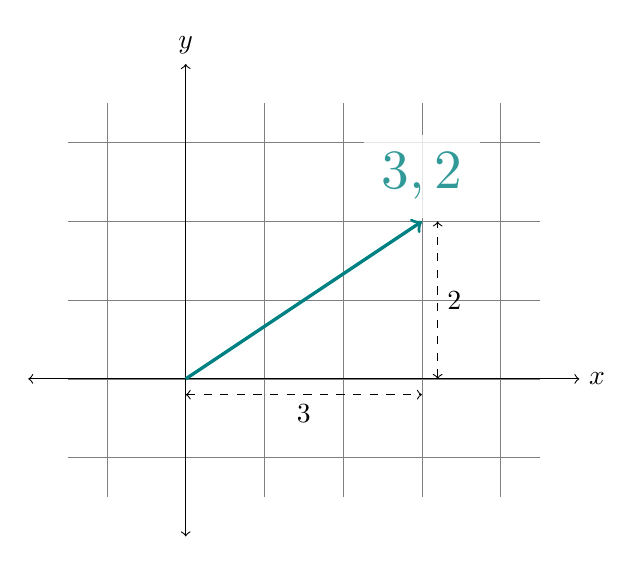
\begin{tikzpicture}
\draw[gray, very thin] (-1.5,-1.5) grid (4.5,3.5);
\draw[<->] (-2,0) -- (5,0) node [pos=1, right] {$x$};
\draw[<->] (0,-2) -- (0,4) node [pos=1, above] {$y$};
\draw[->, very thick, teal] (0,0) -- (3,2) node [fill = white, fill opacity = 0.8, pos=1, above, scale = 2] {$\bv{\red{3},\blue{2}}$};
\draw[<->, dashed] (0,-0.2) -- (3,-0.2) node [pos = 0.5, below] {$\red{3}$};
\draw[<->, dashed] (3.2,0) -- (3.2,2) node [pos = 0.5, right] {$\blue{2}$};
\end{tikzpicture}
\caption{Vector $\bv{3,2}$}
\end{figure}
\end{frame}


\begin{frame}
\begin{figure}[h!]
\centering
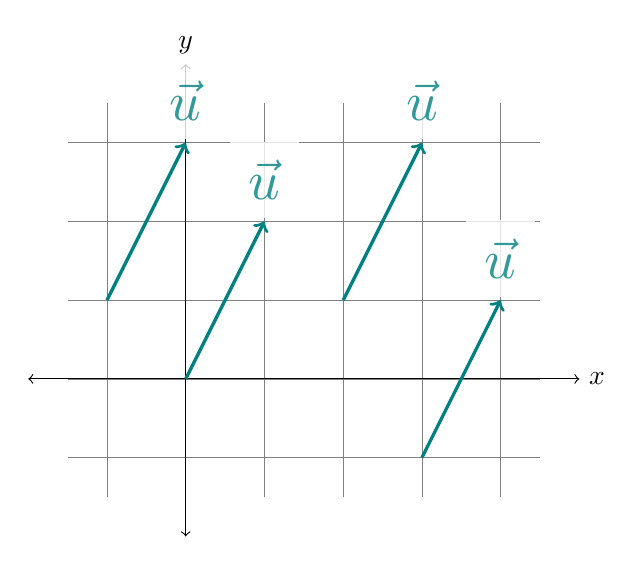
\begin{tikzpicture}
\draw[gray, very thin] (-1.5,-1.5) grid (4.5,3.5);
\draw[<->] (-2,0) -- (5,0) node [pos=1, right] {$x$};
\draw[<->] (0,-2) -- (0,4) node [pos=1, above] {$y$};
\draw[->, very thick, teal] (-1,1) -- (0,3) node [fill = white, fill opacity = 0.8, pos=1, above, scale = 2] {$\vec{u}$};
\draw[->, very thick, teal] (0,0) -- (1,2) node [fill = white, fill opacity = 0.8, pos=1, above, scale = 2] {$\vec{u}$};
\draw[->, very thick, teal] (3,-1) -- (4,1) node [fill = white, fill opacity = 0.8, pos=1, above, scale = 2] {$\vec{u}$};
\draw[->, very thick, teal] (2,1) -- (3,3) node [fill = white, fill opacity = 0.8, pos=1, above, scale = 2] {$\vec{u}$};
\end{tikzpicture}
\caption{A vector $\vec{u}$ may start at any point.}
\end{figure}
\end{frame}

\begin{frame}
\begin{figure}[h!]
\centering
\begin{tikzpicture}
\draw[<->] (0,0) -- (5,0) node [right] {$x$};
\draw[<->] (0,0) -- (-2,-2) node [below left] {$y$};
\draw[<->] (0,0) -- (0,3) node [below left] {$z$};
\draw[->, very thick] (0,0) -- (2.59,1.59) node [above, scale = 2] {$\bv{\red{4},\blue{2},\color{teal}{3}}$};
\draw[->, dashed, red] (0,0) -- (4,0) node [pos = 0.3, below] {4};
\draw[->, dashed, blue] (4,0) -- (2.59,-1.41) node [pos = 0.5, below right] {2};
\draw[->, dashed, teal] (2.59,-1.41) -- (2.59, 1.59) node [pos = 0.8, right] {3};
\end{tikzpicture}
\caption{A 3-dimentional vector $\bv{4,2,3}$}
\end{figure}
\end{frame}


%%%%%%%%%%%%%
\section[Non-origin]{A vector starting from any point}
\frame{\sectionpage}
%%%%%%%%%%%%%

\begin{frame}
\frametitle{A vector starting from a non-origin point}
Sometimes a vector is given as a direction from one point to another. 

\begin{defn}{}{}
Let $P_1(x_1, y_1)$ and $P_2(x_2, y_2)$ be points on the plane. \pa A vector starting at $P_1$ and ending at $P_2$ is denoted by $\vec{P_1P_2}$ \pa which can be computed as follows.
\begin{equation}
\overrightarrow{P_1P_2} \pa = \bv{ x_2 - x_1, y_2 - y_1}
\end{equation} \pa
\end{defn}
\end{frame}


\begin{frame}
\begin{figure}[h!]
\centering
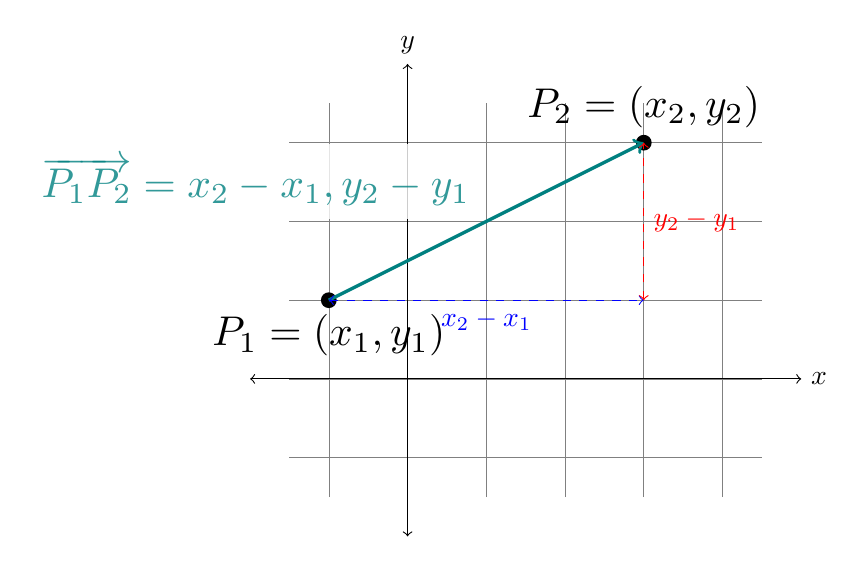
\begin{tikzpicture}
\draw[gray, very thin] (-1.5,-1.5) grid (4.5,3.5);
\draw[<->] (-2,0) -- (5,0) node [pos=1, right] {$x$};
\draw[<->] (0,-2) -- (0,4) node [pos=1, above] {$y$};
\fill (-1,1) circle [radius = 0.1cm] node [scale = 1.5, below] {$P_1 = (x_1, y_1)$};
\fill (3,3) circle [radius = 0.1cm] node [scale = 1.5, above] {$P_2 = (x_2, y_2)$};
\draw[->, very thick, teal] (-1,1) -- (3,3) node [fill = white, fill opacity = 0.8, pos=0.5, above left, scale = 1.5] {$\overrightarrow{P_1P_2} = \bv{ x_2 - x_1, y_2 - y_1}$};
\draw[dashed, <->, blue] (-1,1) -- (3,1) node [below, pos =0.5] {$x_2-x_1$};
\draw[dashed, <->, red] (3,1) -- (3,3) node [right, pos=0.5] {$y_2-y_1$};
\end{tikzpicture}
\caption{A vector from $P_1$ to $P_2$}
\end{figure}
\end{frame}


\begin{frame}[t]
\begin{ex}{}
Find the following vectors
\begin{tasks}(2)
\task $From P_1(3,2)$ to $P_2(4,6)$
\task $From Q_1(-1,0)$ to $Q_2(3,-2)$
\end{tasks}
\end{ex}
\begin{sol}
Directly apply the formula.
\begin{tasks}(1)
\task $\overrightarrow{P_1P_2} \pa = \bv{4-3, 6-2} \pa = \bv{1,4}$ \pa
\task $\overrightarrow{Q_1Q_2} \pa = \bv{3-(-1), -2-0} \pa = \bv{4,-2}$
\end{tasks}
\end{sol}
\end{frame}

%%%%%%%%%%%%%
\section[Operation]{Vector Operations}
\frame{\sectionpage}
%%%%%%%%%%%%%

\begin{frame}
\frametitle{Vector Operations}
Here are some basic vector operations using the new notation.
\begin{defn}{}{}
\begin{itemize}
\item Scalar multiplication: $k\cvec{v_1}{v_2} = \cvec{kv_1}{kv_2}$
\item Addition: $\cvec{v_1}{v_2} + \cvec{u_1}{u_2} = \cvec{v_1 + u_1}{v_2 + u_2}$
\item Subtraction: $\cvec{v_1}{v_2} - \cvec{u_1}{u_2} = \cvec{v_1}{v_2} + \cvec{-u_1}{-u_2} = \cvec{v_1 - u_1}{v_2 - u_2}$
\end{itemize}
\end{defn}
\end{frame}


\begin{frame}
\begin{figure}[h!]
\centering
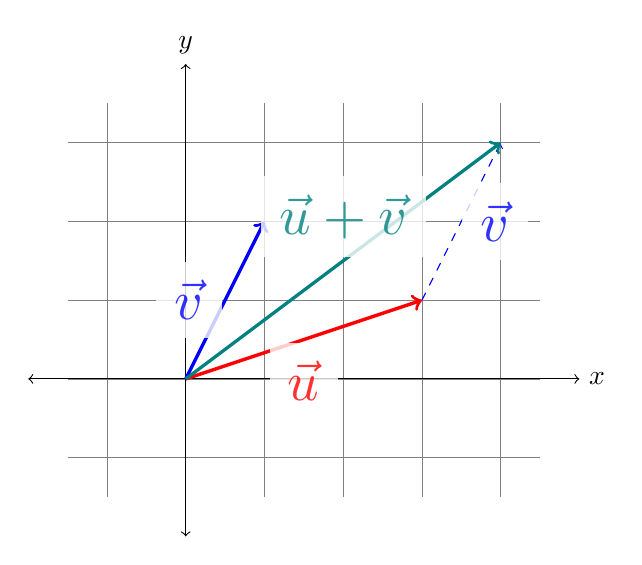
\begin{tikzpicture}
\draw[gray, very thin] (-1.5,-1.5) grid (4.5,3.5);
\draw[<->] (-2,0) -- (5,0) node [pos=1, right] {$x$};
\draw[<->] (0,-2) -- (0,4) node [pos=1, above] {$y$};
\draw[->, very thick, red] (0,0) -- (3,1) node [fill = white, fill opacity = 0.8, pos=0.5, below, scale = 2] {$\vec{u}$};
\draw[->, very thick, blue] (0,0) -- (1,2) node [fill = white, fill opacity = 0.8, pos=0.5, left, scale = 2] {$\vec{v}$};
\draw[->, dashed, blue] (3,1) -- (4,3) node [fill = white, fill opacity = 0.8, pos=0.5, right, scale = 2] {$\vec{v}$};
\draw[->, very thick, teal] (0,0) -- (4,3) node [fill = white, fill opacity = 0.8, pos=0.5, above, scale = 2] {$\vec{u} + \vec{v}$};
\end{tikzpicture}
\caption{Vector addition $\vec{u} + \vec{v}$}
\end{figure}
\end{frame}

\begin{frame}
\begin{figure}[h!]
\centering
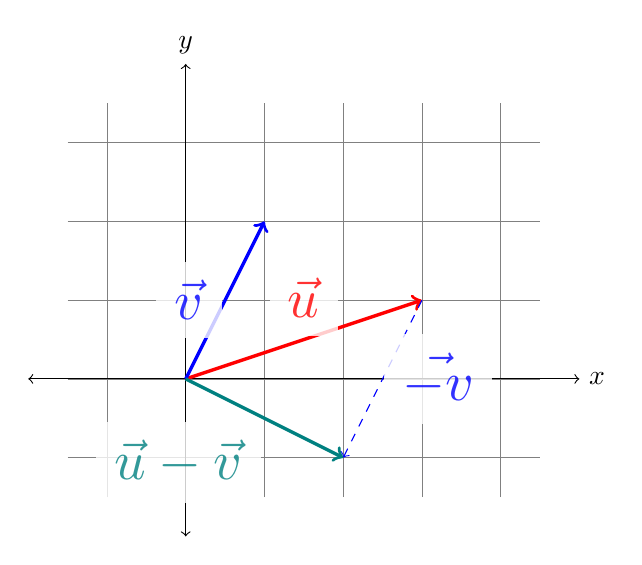
\begin{tikzpicture}
\draw[gray, very thin] (-1.5,-1.5) grid (4.5,3.5);
\draw[<->] (-2,0) -- (5,0) node [pos=1, right] {$x$};
\draw[<->] (0,-2) -- (0,4) node [pos=1, above] {$y$};
\draw[->, very thick, red] (0,0) -- (3,1) node [fill = white, fill opacity = 0.8, pos=0.5, above, scale = 2] {$\vec{u}$};
\draw[->, very thick, blue] (0,0) -- (1,2) node [fill = white, fill opacity = 0.8, pos=0.5, left, scale = 2] {$\vec{v}$};
\draw[->, dashed, blue] (3,1) -- (2,-1) node [fill = white, fill opacity = 0.8, pos=0.5, right, scale = 2] {$\vec{-v}$};
\draw[->, very thick, teal] (0,0) -- (2,-1) node [fill = white, fill opacity = 0.8, pos=0.5, below left, scale = 2] {$\vec{u} - \vec{v}$};
\end{tikzpicture}
\caption{Vector subtraction $\vec{u} - \vec{v}$}
\end{figure}
\end{frame}

\begin{frame}
\begin{figure}[h!]
\centering
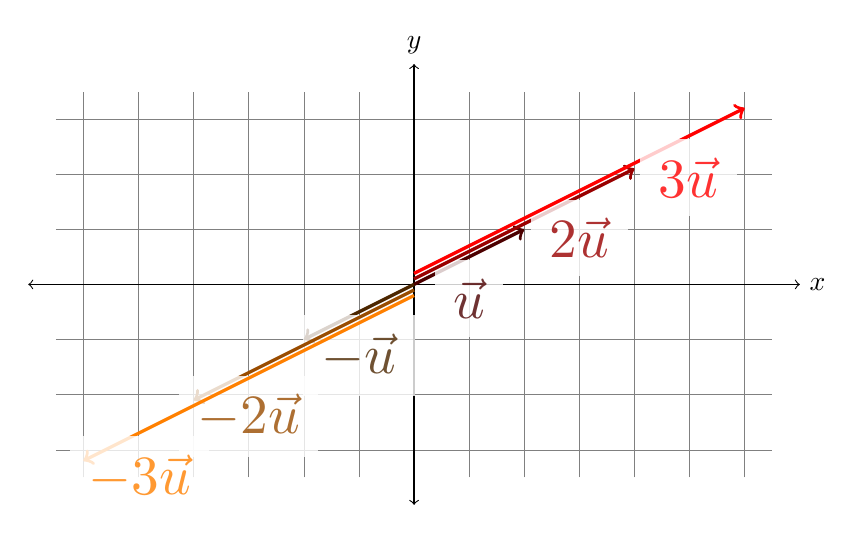
\begin{tikzpicture}[scale =0.7]
\draw[gray, very thin] (-6.5,-3.5) grid (6.5,3.5);
\draw[<->] (-7,0) -- (7,0) node [pos=1, right] {$x$};
\draw[<->] (0,-4) -- (0,4) node [pos=1, above] {$y$};
\draw[->, very thick, red!30!black] (0,0) -- (2,1) node [fill = white, fill opacity = 0.8, pos=0.5, below, scale = 2] {$\vec{u}$};
\draw[->, very thick, red!60!black] (0,0.1) -- (4,2.1) node [fill = white, fill opacity = 0.8, pos=0.75, below, scale = 2] {$2\vec{u}$};
\draw[->, very thick, red] (0,0.2) -- (6,3.2) node [fill = white, fill opacity = 0.8, pos=0.83, below, scale = 2] {$3\vec{u}$};
\draw[->, very thick, orange!30!black] (0,0) -- (-2,-1) node [fill = white, fill opacity = 0.8, pos=0.5, below, scale = 2] {$-\vec{u}$};
\draw[->, very thick, orange!60!black] (0,-0.1) -- (-4,-2.1) node [fill = white, fill opacity = 0.8, pos=0.75, below, scale = 2] {$-2\vec{u}$};
\draw[->, very thick, orange] (0,-0.2) -- (-6,-3.2) node [fill = white, fill opacity = 0.8, pos=0.83, below, scale = 2] {$-3\vec{u}$};
\end{tikzpicture}
\caption{Scalar multiplication $k\vec{u}$ when $k$ is $-3,-2,-1,1,2$ and $3$}
\end{figure}
\end{frame}

\begin{frame}
\frametitle{Basic Properties}
\begin{prop}{}{}
\begin{itemize}
\item Distribution: $a (\vec{v} + \vec{w}) = a\vec{v} + a\vec{w}$
\item Distribution: $(a+b)\vec{v} = a\vec{v} + b\vec{v}$
\item Identity: $1\vec{v} = \vec{v}$
\item Define $\vec{0} = \cvec{0}{0}$. Then, we have 
\[\vec{v} + \vec{0} = \vec{0} + \vec{v} = \vec{v}\]
\item $(-1)\vec{v} = -\vec{v}$
\item If $\vec{v} = a \vec{w}$ then we say that $\vec{v}$ and $\vec{w}$ are parallel.
\end{itemize}
\end{prop}
\end{frame}

%%%%%%%%%%%%%
\section[Norm and Unit] {Norm and Unit Vectors}
\frame{\sectionpage}
%%%%%%%%%%%%%

\begin{frame}
\frametitle{Vector Norm}
Since a vector, drawn as an arrow, has length, then we can compute it using Pythagoras' Theorem.
\begin{defn}{}{}
The \textbf{norm} (or length) of a vector $\vec{v} = \cvec{a}{b}$ is 
\begin{equation}
\| \vec{v} \| = \sqrt{a^2+b^2}
\end{equation}
\end{defn}
\end{frame}

\begin{frame}
\begin{figure}[h!]
\centering
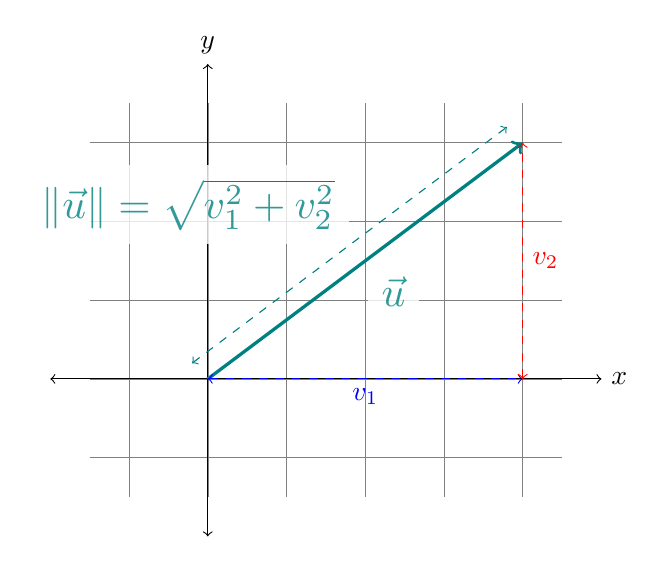
\begin{tikzpicture}
\draw[gray, very thin] (-1.5,-1.5) grid (4.5,3.5);
\draw[<->] (-2,0) -- (5,0) node [pos=1, right] {$x$};
\draw[<->] (0,-2) -- (0,4) node [pos=1, above] {$y$};
\draw[->, very thick, teal] (0,0) -- (4,3) node [fill = white, fill opacity = 0.8, pos=0.5, below right, scale = 1.5] {$\vec{u}$};
\draw[<->, dashed, teal] (-0.2,0.2) -- (3.8,3.2) node [fill = white, fill opacity = 0.8, pos=0.5, above left, scale = 1.5] {$\| \vec{u} \| = \sqrt{v_1^2 + v_2^2}$};
\draw[<->, dashed, blue] (0,0) -- (4,0) node [below, pos =0.5] {$v_1$};
\draw[<->, dashed, red] (4,0) -- (4,3) node [right, pos=0.5] {$v_2$};
\end{tikzpicture}
\caption{Norm of vector $\vec{u}$}
\end{figure}
\end{frame}



\begin{frame}{Unit Vector}
\begin{defn}{}{}
A unit vector $\vec{u}$ is a vector with norm equal to 1 ($\| \vec{u} \| = 1$).
\end{defn}
\begin{figure}[h!]
\centering
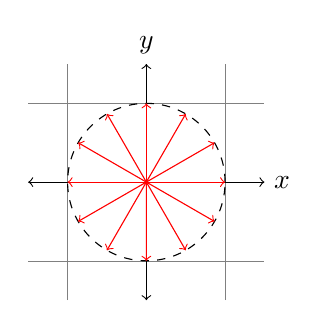
\begin{tikzpicture}
\draw[gray, very thin] (-1.5,-1.5) grid (1.5,1.5);
\draw[<->] (-1.5,0) -- (1.5,0) node [pos=1, right] {$x$};
\draw[<->] (0,-1.5) -- (0,1.5) node [pos=1, above] {$y$};
\draw[dashed] (0,0) circle [radius = 1cm];
\foreach \r in {0,1,...,11}
{
	\draw[->, red] (0,0) -- (\r*pi/6 r: 1cm);
}
\end{tikzpicture}
\caption{Unit vectors }
\end{figure}
\end{frame}


\begin{frame}
\frametitle{The Standard Unit Vectors}
\begin{defn}{}{}
The standard unit vectors in two dimension $\textbf{i}$ and $\textbf{j}$ are defined as
\[ \textbf{i} = \cvec{1}{0}, \qquad \textbf{j} = \cvec{0}{1}.\]

\tcblower
Given a vector $\vec{v} = \cvec{v_1}{v_2}$, we can rewrite $\vec{v}$ as 
\[ \vec{v} = v_1 \textbf{i} + v_2 \textbf{j}\]
\end{defn}
\end{frame}

\begin{frame}
\begin{figure}[h!]
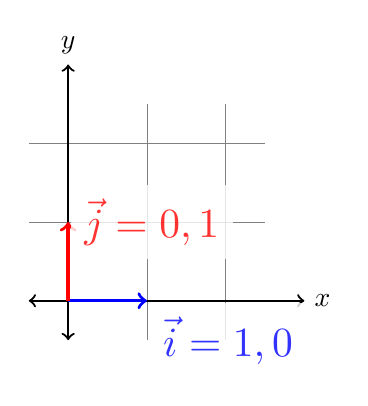
\begin{tikzpicture}
\draw[very thin,color=gray] (-0.5,-0.5) grid (2.5,2.5);
\draw[<->, thick] (-0.5,0) -- (3,0) node[right] {$x$};
\draw[<->, thick] (0,-0.5) -- (0,3) node[above] {$y$};
\draw[->, blue, very thick] (0,0) -- (1,0) node[below right, scale = 1.5, fill = white, fill opacity = 0.8] {$\vec{i} = \bv{1,0}$};
\draw[->, red, very thick] (0,0) -- (0,1) node[right, scale = 1.5, fill = white, fill opacity = 0.8] {$\vec{j} = \bv{0,1}$};
\end{tikzpicture}
\caption{The unit vectors $\vec{i}$ and $\vec{j}$}

We can express $\vec{v}$ as a linear combination of $\vec{i}$ and $\vec{j}$ as
\[ \vec{v} = \bv{v_1, v_2} \pa = \vv{v_1}{+ v_2}\]
\end{figure}
\end{frame}

\begin{frame}[t]
\begin{ex}{}
Express the following vectors as a linear combination of $\vec{i}$ and $\vec{j}$ 
\begin{tasks}(2)
\task $\bv{3,4} $
\task $\bv{-2,2}$
\task $\bv{0,-2}$
\task $\bv{5,0}$
\end{tasks}
\end{ex}
\begin{sol}
\begin{tasks}(1)
\task $\bv{3,4} \pa = \vv{3}{+4}$ \pa
\task $\bv{-2,2} \pa= \vv{-2}{+2}$ \pa
\task $\bv{0,-2} \pa= -2 \bvec{j}$ \pa
\task $\bv{5,0} \pa = 5\bvec{i}$
\end{tasks}
\end{sol}
\end{frame}


\begin{frame}[t]
\begin{ex}{}
Express the following vectors as $\langle , \rangle$
\begin{tasks}(2)
\task $\vv{2}{-5} $
\task $\vv{-1}{2}$
\task $3\bvec{i}$
\task $-4\bvec{j}$
\end{tasks}
\end{ex}
\begin{sol}
\begin{tasks}(1)
\task $\vv{2}{-5} \pa = \bv{2,-5}$ \pa
\task $\vv{-1}{2} \pa = \bv{-1,2}$ \pa
\task $3\bvec{i} \pa = 3\bvec{i} + 0\bvec{j} \pa = \bv{3,0}$ \pa
\task $-4\bvec{j} = 0\bvec{i} - 4\bvec{j} = \bv{0,-4}$
\end{tasks}
\end{sol}
\end{frame}

%%%%%%%%%%%%%
\section{Dot Product}
\frame{\sectionpage}
%%%%%%%%%%%%%

\begin{frame}
So far, we know how to multiply a scalar to a vector, but can we multiply a vector to another vector?
\frametitle{Dot Product}
\begin{defn}{}{}
Given vectors $\vec{v} = \cvec{a}{b}$ and $\vec{w} = \cvec{c}{d}$, the \textbf{dot product} is 
\begin{equation}
\vec{v} \cdot \vec{w} = ac + bd
\end{equation}
\end{defn}
Note that the result is a \textbf{scalar}, not a \textbf{vector}!
\end{frame}


\begin{frame}[t]
\begin{ex}{}
Compute the dot products.
\begin{tasks}(2)
\task $\bv{3,4} \cdot \bv{1,2}$
\task $\bv{-2,2} \cdot \bv{-2,1}$
\task $\bv{0,3} \cdot \bv{9,0}$
\task $\bv{2,-2,1} \cdot \bv{1,1,3}$
\end{tasks}
\end{ex}
\begin{sol}
\begin{tasks}(1)
\task $\bv{3,4} \cdot \bv{1,2} \pa = (3 \times 1) \pa + (4 \times 2) \pa = 3 + 8 \pa = 11$ \pa
\task $\bv{-2,2} \cdot \bv{-2,1} \pa = ((-2) \times (-2)) \pa + (2 \times 1) \pa = 4 + 2 \pa = 6$ \pa
\task  $\bv{0,3} \cdot \bv{9,0} \pa = (0 \times 9) + (3 \times 0) \pa = 0 + 0 \pa = 0$ \pa
\task $\bv{2,-2,1} \cdot \bv{1,1,3} \pa = (2 \times 1) \pa + ((-2) \times 1) \pa + (1 \times 3) \pa = 2 + (-2) + 3 \pa = 3$
\end{tasks}
\end{sol}
\end{frame}

\begin{frame}{Dot product application}
Why is the dot product defined this way? One reason is that the formula will be useful in other applications. For instance, we have the following theorem.

\begin{thm}{}{}
Given vectors $\vec{v}, \vec{u}$ and let $\theta$ be the angle between both vectors. Then,
\[ \cos \theta = \frac{\vec{v} \cdot \vec{u}}{\| \vec{v} \| \| \vec{u} \|}\]
\end{thm}

Then, using this application, we can view the dot product as the product of the length of vectors after one vector is projected onto the other vector.
\end{frame}

\begin{frame}
\frametitle{Angel between vectors}
\begin{defn}{}{}
Given vectors $\vec{u}$ and $\vec{v}$, then the angle $\theta$ between vectors is the angle measured when both vectors start at the origin such that $0 \leq \theta \leq \pi$.
\end{defn}

\begin{figure}[h!]
\centering
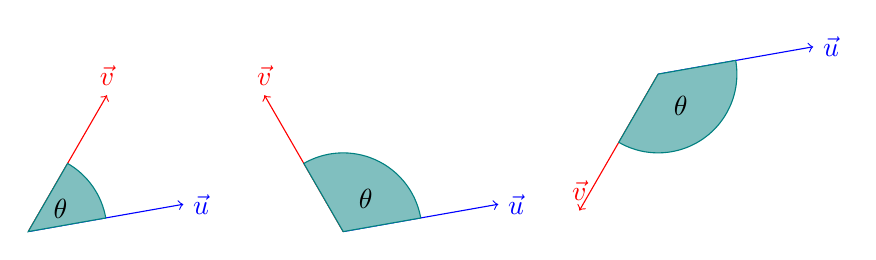
\begin{tikzpicture}
\draw[->, blue] (0,0) -- (10:2) node [right] {$\vec{u}$};
\draw[->, red] (0,0) -- (60:2) node [above] {$\vec{v}$};
\filldraw[fill = teal!50!white, draw = teal] (0,0) -- (10:1) arc [start angle = 10, end angle = 60, radius = 1] -- cycle;
\node at (35:0.5) {$\theta$};
\begin{scope}[xshift = 4cm]
\draw[->, blue] (0,0) -- (10:2) node [right] {$\vec{u}$};
\draw[->, red] (0,0) -- (120:2) node [above] {$\vec{v}$};
\filldraw[fill = teal!50!white, draw = teal] (0,0) -- (10:1) arc [start angle = 10, end angle = 120, radius = 1] -- cycle;
\node at (55:0.5) {$\theta$};
\end{scope}
\begin{scope}[xshift = 8cm, yshift = 2cm]
\draw[->, blue] (0,0) -- (10:2) node [right] {$\vec{u}$};
\draw[->, red] (0,0) -- (240:2) node [above] {$\vec{v}$};
\filldraw[fill = teal!50!white, draw = teal] (0,0) -- (240:1) arc [start angle = 240, end angle = 370, radius = 1] -- cycle;
\node at (305:0.5) {$\theta$};
\end{scope}
\end{tikzpicture}
\caption{Angle $\theta$ between $\vec{u}$ and $\vec{v}$}
\end{figure}
\end{frame}

\begin{frame}
\begin{thm}{}{}
Let $\theta$ be the angle between $\vec{u}$ and $\vec {v}$ then 
\begin{equation}
\cos \theta = \frac{\vec{u} \cdot \vec{v} }{\| \vec{u} \|\| \vec{v} \|.}
\end{equation} \pa
Consequently, we have
\begin{equation}
\theta = \arccos \left( \frac{\vec{u} \cdot \vec{v} }{\| \vec{u} \|\| \vec{v} \|} \right), \quad 0 \leq \theta \leq \pi.
\end{equation}
\end{thm}
\end{frame}

 
\begin{frame}[t]
\begin{ex}{}
Find the angle $\theta$ between $\bv{1,4}$ and $\bv{4,1}$
\end{ex}
\begin{sol} Compute the dot product and norms. \pa
\begin{eq*} 
\| \bv{1,4} \| \pa &=& \sqrt{1^2+4^2} = \sqrt{17} \pa \\
\| \bv{4,1} \| \pa &=& \sqrt{4^2+1^2} = \sqrt{17} \pa \\
\bv{1,4} \cdot \bv{4,1} \pa &=& (1\times 4) + (4 \times 1) = 8
\end{eq*}
Then, \pa

\[\cos \theta = \frac{\vec{u} \cdot \vec{v} }{\| \vec{u} \|\| \vec{v} \|} \pa = \frac{8}{\sqrt{17}\times \sqrt{17}} \pa = \frac{8}{17}\]
Therefore, $\theta = \arccos \left( \frac{8}{17} \right)$
\end{sol}
\end{frame}

\begin{frame}[t]
This gives us an application of the dot product.
\begin{slide}
\begin{thm}{}{}
Given vectors $\vec{u}$ and $\vec{v}$ such that $\vec{u} \neq \vec{0}$ and $\vec{v} \neq \vec{0}$  where $\theta$ is the angle between the vectors. \pa
\begin{itemize}
\item If $\vec{u} \cdot \vec{v} = 0$ \pa, then $\theta = \tfrac{\pi}{2}$ implying that they are perpendicular to each other. We denote this as $\vec{u} \perp \vec{v}$. \pa
\item If $\vec{u} \cdot \vec{v} > 0$ \pa, then $\theta$ is an acute angle ($0 \leq \theta < \tfrac{\pi}{2}$) \pa
\item If $\vec{u} \cdot \vec{v} < 0$ \pa, then $\theta$ is an obtuse angle ($\tfrac{\pi}{2} < \theta \leq \pi$) \pa
\end{itemize}
\end{thm}
\end{slide}
\end{frame}



\iffalse
\begin{frame}
\begin{exercisebox}{}{}
\begin{enumerate}
\item Simplify the following expressions.
\begin{tasks}(3)
\task $ \cvec{1}{2} + \cvec{3}{4}$
\task $ 3\cvec{2}{1}$
\task $ (-2)\cvec{1}{-4}$
\end{tasks}

\item Compute the norm of these vectors.
\begin{tasks}(3)
\task $ \cvec{0}{2}$
\task $\cvec{3}{4}$
\task $\cvec{-2}{1}$
\end{tasks}

\item Compute the dot products.
\begin{tasks}(2)
\task $ \cvec{1}{2} \cdot \cvec{3}{4}$
\task $ \cvec{-2}{1} \cdot \cvec{5}{+6}$
\end{tasks}
\end{enumerate}
\end{exercisebox}
\end{frame}
\fi


%%%%%%%%%%%%%
\section[2D on plane]{2D Transformation on the Plane}
\frame{\sectionpage}
%%%%%%%%%%%%%

\begin{frame}
\addfig{0.7}{2dtransform_golf}{\href{https://teacher.desmos.com/activitybuilder/custom/59b01d08f4d48d0a0ee7526e}{Click here to play Golf!}}{}
\end{frame}

\begin{frame}
\frametitle{Analytical Approach}
Consider a plane that consists of all points $(x,y)$ where $x,y$ are real numbers.

We think of 2D transformation as a function 
\[ T(\vec{v}) = \vec{v}'\]
In other words,
\[\cvec{v_1}{v_2} \to \cvec{v_1'}{v_2'}\]
where $v_1, v_2, v_1', v_2'$ are real numbers.
\end{frame}


\begin{frame}[t]
\begin{ex}
Describe how each transformation change the square consisting of points $(0,0), (0,1), (1,1)$ and $(1,0)$.
\begin{tasks}(2)
\task $\cvec{x}{y} \to \cvec{2x}{y}$
\task $\cvec{x}{y} \to \cvec{x}{-2y}$
\task $\cvec{x}{y} \to \cvec{y}{-x}$
\task $\cvec{x}{y} \to \cvec{x+y}{x-y}$
\end{tasks}
\end{ex}
\end{frame}

\begin{frame}
\begin{sol}
(a) Compute the image of transformation of each point. 
\[\green{\cvec{0}{0} \to \cvec{0}{0}}  \qquad 
\textcolor{yellow}{\cvec{1}{0} \to \cvec{2}{0}} \qquad
\blue{\cvec{1}{1} \to \cvec{2}{1}}  \qquad 
\red{\cvec{0}{1} \to \cvec{0}{1}} \]

\begin{figure}[h!]
\centering
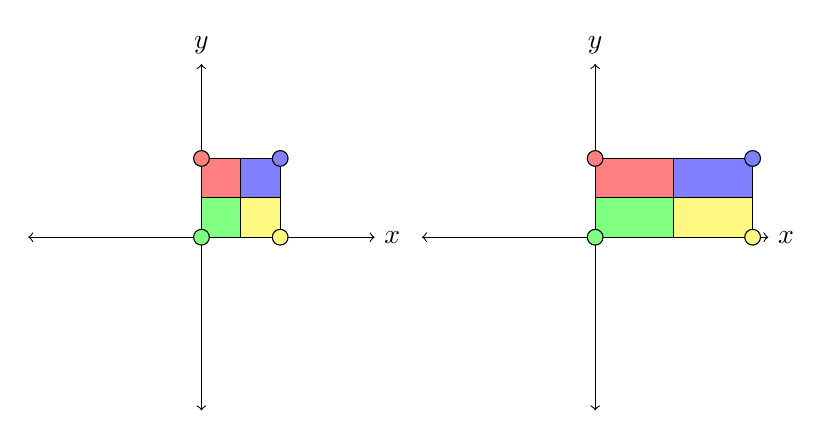
\begin{tikzpicture}[draw = black]
\draw[<->] (-2.2,0) -- (2.2,0) node [right] {$x$};
\draw[<->] (0,-2.2) -- (0,2.2) node [above] {$y$};
\filldraw[fill = green!50] (0,0) rectangle (0.5,0.5);
\filldraw[fill = green!50] (0,0) circle (0.1cm);
\filldraw[fill = yellow!50] (0.5,0) rectangle (1,0.5);
\filldraw[fill = yellow!50] (1,0) circle (0.1cm);
\filldraw[fill = blue!50] (0.5,0.5) rectangle (1,1);
\filldraw[fill = blue!50](1,1) circle (0.1cm);
\filldraw[fill = red!50] (0,0.5) rectangle (0.5,1);
\filldraw[fill = red!50] (0,1) circle (0.1cm);
\begin{scope}[xshift = 5cm]
\draw[<->] (-2.2,0) -- (2.2,0) node [right] {$x$};
\draw[<->] (0,-2.2) -- (0,2.2) node [above] {$y$};
\filldraw[fill = green!50] (0,0) rectangle (1,0.5);
\filldraw[fill = green!50] (0,0) circle (0.1cm);
\filldraw[fill = yellow!50] (1,0) rectangle (2,0.5);
\filldraw[fill = yellow!50] (2,0) circle (0.1cm);
\filldraw[fill = blue!50] (1,0.5) rectangle (2,1);
\filldraw[fill = blue!50] (2,1) circle (0.1cm);
\filldraw[fill = red!50] (0,0.5) rectangle (1,1);
\filldraw[fill = red!50] (0,1) circle (0.1cm);
\end{scope}
\end{tikzpicture}
\end{figure}
This is a dilation in the x-axis by a factor of 2.
\end{sol}
\end{frame}

\begin{frame}
\begin{sol}
(b)
\[\green{\cvec{0}{0} \to \cvec{0}{0}} \qquad 
\textcolor{yellow}{\cvec{1}{0} \to \cvec{1}{0}} \qquad
\blue{\cvec{1}{1} \to \cvec{1}{-2}} \qquad 
\red{\cvec{0}{1} \to \cvec{0}{-2}}\] 
\begin{figure}
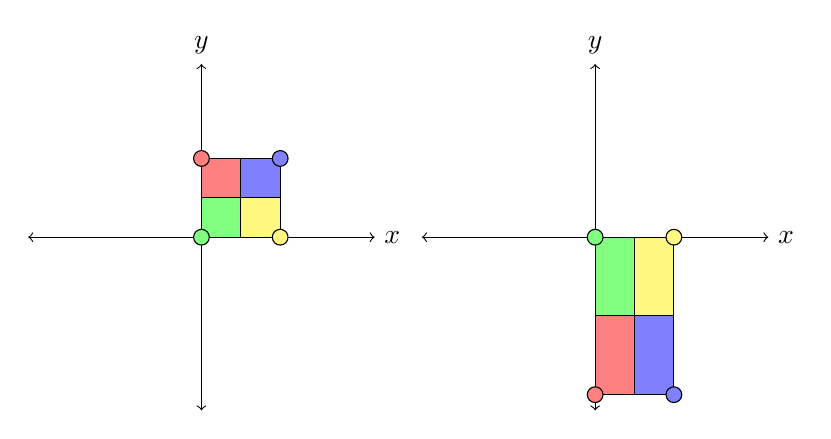
\begin{tikzpicture}[draw = black]
\draw[<->] (-2.2,0) -- (2.2,0) node [right] {$x$};
\draw[<->] (0,-2.2) -- (0,2.2) node [above] {$y$};
\filldraw[fill = green!50] (0,0) rectangle (0.5,0.5);
\filldraw[fill = green!50] (0,0) circle (0.1cm);
\filldraw[fill = yellow!50] (0.5,0) rectangle (1,0.5);
\filldraw[fill = yellow!50] (1,0) circle (0.1cm);
\filldraw[fill = blue!50] (0.5,0.5) rectangle (1,1);
\filldraw[fill = blue!50](1,1) circle (0.1cm);
\filldraw[fill = red!50] (0,0.5) rectangle (0.5,1);
\filldraw[fill = red!50] (0,1) circle (0.1cm);
\begin{scope}[xshift = 5cm]
\draw[<->] (-2.2,0) -- (2.2,0) node [right] {$x$};
\draw[<->] (0,-2.2) -- (0,2.2) node [above] {$y$};
\filldraw[fill = green!50] (0,0) rectangle (0.5,-1);
\filldraw[fill = green!50] (0,0) circle (0.1cm);
\filldraw[fill = yellow!50] (0.5,0) rectangle (1,-1);
\filldraw[fill = yellow!50]  (1,0) circle (0.1cm);
\filldraw[fill = blue!50] (0.5,-1) rectangle (1,-2);
\filldraw[fill = blue!50] (1,-2) circle (0.1cm);
\filldraw[fill = red!50] (0,-1) rectangle (0.5,-2);
\filldraw[fill = red!50] (0,-2) circle (0.1cm);
\end{scope}
\end{tikzpicture}
\end{figure}
This is a dilation in the y-axis by a factor of -2.
\end{sol}
\end{frame}

\begin{frame}
\begin{sol}
(c)
\[\green{\cvec{0}{0} \to \cvec{0}{0}} \qquad 
\textcolor{yellow}{\cvec{1}{0} \to \cvec{0}{-1}} \qquad
\blue{\cvec{1}{1} \to \cvec{-1}{1}} \qquad 
\red{\cvec{0}{1} \to \cvec{-1}{0}} \]
\begin{figure}[h!]
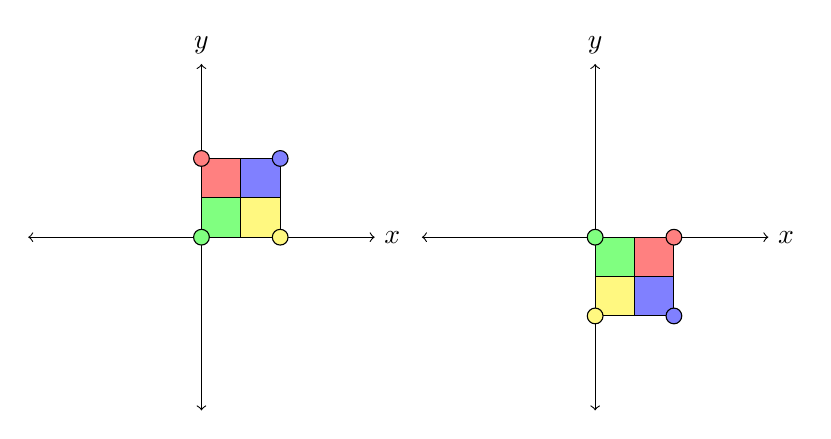
\begin{tikzpicture}[draw = black]
\draw[<->] (-2.2,0) -- (2.2,0) node [right] {$x$};
\draw[<->] (0,-2.2) -- (0,2.2) node [above] {$y$};
\filldraw[fill = green!50] (0,0) rectangle (0.5,0.5);
\filldraw[fill = green!50] (0,0) circle (0.1cm);
\filldraw[fill = yellow!50] (0.5,0) rectangle (1,0.5);
\filldraw[fill = yellow!50] (1,0) circle (0.1cm);
\filldraw[fill = blue!50] (0.5,0.5) rectangle (1,1);
\filldraw[fill = blue!50](1,1) circle (0.1cm);
\filldraw[fill = red!50] (0,0.5) rectangle (0.5,1);
\filldraw[fill = red!50] (0,1) circle (0.1cm);
\begin{scope}[xshift = 5cm]
\draw[<->] (-2.2,0) -- (2.2,0) node [right] {$x$};
\draw[<->] (0,-2.2) -- (0,2.2) node [above] {$y$};
\filldraw[fill = green!50] (0,0) rectangle (0.5,-0.5);
\filldraw[fill = green!50] (0,0) circle (0.1cm);
\filldraw[fill = yellow!50] (0,-0.5) rectangle (0.5,-1);
\filldraw[fill = yellow!50] (0,-1) circle (0.1cm);
\filldraw[fill = blue!50] (0.5,-0.5) rectangle (1,-1);
\filldraw[fill = blue!50] (1,-1) circle (0.1cm);
\filldraw[fill = red!50] (0.5,0) rectangle (1,-0.5);
\filldraw[fill = red!50] (1,0) circle (0.1cm);
\end{scope}
\end{tikzpicture}
\end{figure}
This is a rotation around the origin $(0,0)$ by 90 degrees.
\end{sol}
\end{frame}

\begin{frame}
\begin{sol}
(d)
\[\green{\cvec{0}{0} \to \cvec{0}{0}} \qquad 
\textcolor{yellow}{\cvec{1}{0} \to \cvec{1}{1}} \qquad
\blue{\cvec{1}{1} \to \cvec{2}{0}} \qquad 
\red{\cvec{0}{1} \to \cvec{1}{-1}} \]
\begin{figure}[h!]
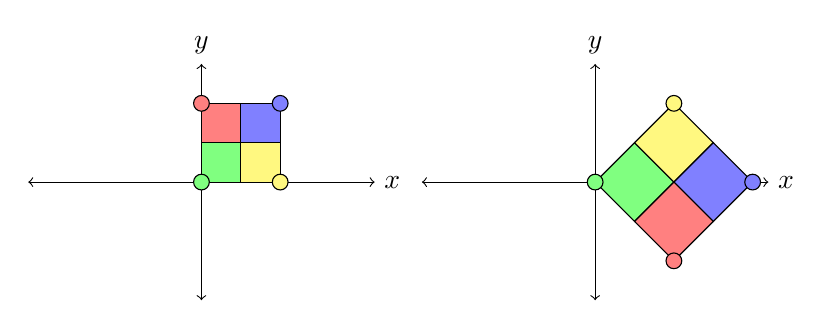
\begin{tikzpicture}[draw = black]
\draw[<->] (-2.2,0) -- (2.2,0) node [right] {$x$};
\draw[<->] (0,-1.5) -- (0,1.5) node [above] {$y$};
\filldraw[fill = green!50] (0,0) rectangle (0.5,0.5);
\filldraw[fill = green!50] (0,0) circle (0.1cm);
\filldraw[fill = yellow!50] (0.5,0) rectangle (1,0.5);
\filldraw[fill = yellow!50] (1,0) circle (0.1cm);
\filldraw[fill = blue!50] (0.5,0.5) rectangle (1,1);
\filldraw[fill = blue!50](1,1) circle (0.1cm);
\filldraw[fill = red!50] (0,0.5) rectangle (0.5,1);
\filldraw[fill = red!50] (0,1) circle (0.1cm);
\begin{scope}[xshift = 5cm]
\draw[<->] (-2.2,0) -- (2.2,0) node [right] {$x$};
\draw[<->] (0,-1.5) -- (0,1.5) node [above] {$y$};
\filldraw[fill = green!50] (0,0) --++ (0.5,0.5) --++ (0.5, -0.5) --++ (-0.5, -0.5) --++ (-0.5, 0.5);
\filldraw[fill = green!50] (0,0) circle (0.1cm);
\filldraw[fill = yellow!50] (0.5,0.5) --++ (0.5,0.5) --++ (0.5, -0.5) --++ (-0.5, -0.5) --++ (-0.5, 0.5);
\filldraw[fill = yellow!50] (1,1) circle (0.1cm);
\filldraw[fill = blue!50] (1,0) --++ (0.5,0.5) --++ (0.5, -0.5) --++ (-0.5, -0.5) --++ (-0.5, 0.5)  ;
\filldraw[fill = blue!50](2,0) circle (0.1cm);
\filldraw[fill = red!50] (0.5,-0.5) --++ (0.5,0.5) --++ (0.5, -0.5) --++ (-0.5, -0.5) --++ (-0.5, 0.5);
\filldraw[fill = red!50] (1,-1) circle (0.1cm);
\end{scope}
\end{tikzpicture}
\end{figure}
This is a rotation around the origin $(0,0)$ by 45 degree, and also a dilation in both directions by a factor of $\sqrt{2}$.
\end{sol}
\end{frame}
\begin{frame}
\begin{exercisebox}{}{}
Describe how each transformation change the square consisting of points $(0,0), (0,1), (1,1)$ and $(1,0)$. Also, explain in your own words what kind of transformation it looks like.
\begin{tasks}(1)
\task $\cvec{x}{y} \to \cvec{3x}{2y}$
\task $\cvec{x}{y} \to \cvec{-x}{2y}$
\task $\cvec{x}{y} \to \cvec{4-x}{2-y}$
\end{tasks}
\end{exercisebox}
\end{frame}

%%%%%%%%%%%%%
\section[Transformation]{Types of Linear Transformations}
\frame{\sectionpage}
%%%%%%%%%%%%%

\begin{frame}
Notice how each of the transformations in the previous example has the form $\cvec{x}{y} \to \cvec{ax+by}{cx+dy}$. This is called a \textbf{linear transformation}.
\begin{remark}{Note}
Informally, a linear transformation $T$ has two properties
\begin{itemize}
\item $T(x+y) = T(x) + T(y)$.
\item $T(cx) = cT(x)$.
\end{itemize}
Given these properties, we can prove all the useful formulas. But we are not going into details here.
\end{remark}
\end{frame}


\begin{frame}
\frametitle{Translation}
\begin{defn}{}{}
A translation by a vector $\vec{a}$ is defined as
\[ T(\vec{v}) = \vec{v} + \vec{a}.\]
In two dimensions, we have
\[ \cvec{v_1}{v_2} \to \cvec{v_1+a_1}{v_2+a_2}.\]
\end{defn}
\end{frame}

\begin{frame}
\frametitle{Dilation (Scaling)}
\begin{defn}{}{}
A dilation by a factor $\vec{k}$ is defined as
\[ T(\vec{v}) = k \cdot \vec{v}.\]
In two dimensions, we have
\[ \cvec{v_1}{v_2} \to \cvec{kv_1}{kv_2}\]
\end{defn}
Note that dilation is the same as scaling up or down, plus reversing if $k$ is negative.
\end{frame}

\begin{frame}
\frametitle{Reflection over a point}
\begin{defn}{}{}
A reflection around a vector $\vec{a} = \cvec{a_1}{a_2}$ (or a point $(a_1, a_2)$) is defined as
\[ T(\vec{v}) = 2\vec{a} - \vec{v}.\]
In two dimensions, we have
\[ \cvec{v_1}{v_2} \to \cvec{2a_1-v_1}{2a_2-v_2}\]
\end{defn}
\end{frame}

\begin{frame}
\frametitle{Rotation}
We can use trigonometry functions and some analysis to compute the formula for rotation, which is.
\[ \cvec{v_1}{v_2} \to \cvec{v_1\cos\theta - v_2\sin\theta}{v_1\sin\theta + v_2\cos\theta}\]
However, it seems impossible to express the result as a linear combination of vectors...
\[ \vec{v} \to ???\]
\end{frame}

\begin{frame}
We can't define rotation using only vector notations. This means that we need to extent the definitions. Notice that
\begin{eq*} 
\cvec{x\cos\theta - y\sin\theta}{ x\sin\theta + y\cos\theta} &=& \cvec{x\cos\theta}{x\cos\theta} + \cvec{-y\sin\theta}{y\cos\theta} \\
&=& x\cvec{\cos\theta}{\sin\theta} + y\cvec{-\sin\theta}{\cos\theta}
\end{eq*}
We'll see how to express the result neatly next week! Stay tuned!
\end{frame}

\begin{frame}
\begin{exercisebox}{}{}
Without computing or graphing, identify the following transformations.
\begin{tasks}(1)
\task $\cvec{x}{y} \to \cvec{2x}{2y}$
\task $\cvec{x}{y} \to \cvec{x+3}{y-2}$
\task $\cvec{x}{y} \to \cvec{1-x}{1-y}$
\end{tasks}
\end{exercisebox}
\end{frame}

